\documentclass[tikz,border=5pt]{standalone}
\usepackage{pgfplots}
\pgfplotsset{compat=1.17}
\usepackage{tikz}
\usetikzlibrary{decorations.pathreplacing,arrows.meta}

% Definición de colores personalizados
\definecolor{lila}{RGB}{152,78,163}
\definecolor{amarillo}{RGB}{255,127,0}

\begin{document}
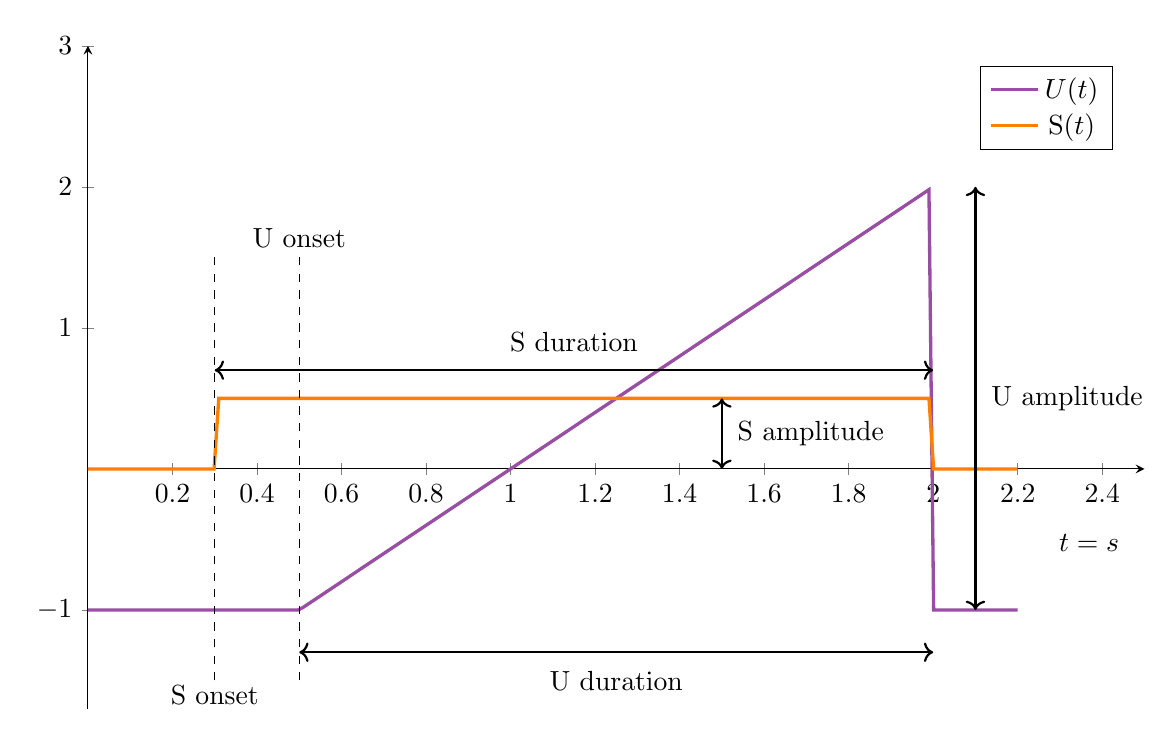
\begin{tikzpicture}

  \pgfmathsetmacro{\Uonset}{0.5}
  \pgfmathsetmacro{\Uoffset}{1.5}
  \pgfmathsetmacro{\Uamp}{3}
  \pgfmathsetmacro{\Stimonset}{0.30}
  \pgfmathsetmacro{\Stimoffset}{1.7}
  \pgfmathsetmacro{\Stimamp}{0.5}

  \begin{axis}[
    width=15cm, height=10cm,
    domain=0:2.2,
    samples=200,
    xmin=0, xmax=2.5,
    ymin=-1.7, ymax=3,
    axis lines=middle,
    xlabel={$t = s$},
    ylabel={},
    legend pos= north east,
    every axis x label/.style={at={(axis description cs:0.91,0.25)},anchor=west},
    every axis y label/.style={at={(axis description cs:0.05,0.95)},anchor=south},
  ]

    % U_t(t) con color lila
    \addplot[lila, very thick] 
      ({x}, { x<\Uonset || x>\Uonset+\Uoffset 
               ? -1 
               : -1 + \Uamp*(x-\Uonset)/\Uoffset });
    \addlegendentry{$U(t)$}

    % S(t) con color amarillo
    \addplot[amarillo, very thick]
      ({x}, { x<\Stimonset || x>\Stimonset+\Stimoffset 
               ? 0 
               : \Stimamp });
    \addlegendentry{$\mathrm{S}(t)$}

    % Onsets (vertical)
    \draw[black, dashed]
      (axis cs:\Uonset,-1.5) -- (axis cs:\Uonset,1.5)
      node[above,pos=1] {U onset};
    \draw[black, dashed]
      (axis cs:\Stimonset,-1.5) -- (axis cs:\Stimonset,1.5)
      node[below,pos=0.01] {S onset};

    % Offsets (horizontales)
    \draw[<->, thick]
      (axis cs:\Uonset,-1.3) -- node[below=3pt] {U duration}(axis cs:{\Uonset+\Uoffset},-1.3);
    \draw[<->, thick]
      (axis cs:\Stimonset,0.7) -- node[above=3pt] {S duration}(axis cs:{\Stimonset+\Stimoffset},0.7);

    % Amplitudes (flechas verticales)
    % U amplitude between baseline and peak
    \draw[<->, thick]
      (axis cs:2.1,-1) -- node[right=2pt] {U amplitude }(axis cs:2.1,{-1+\Uamp});
    % stim amplitude between baseline (0) y top (0.5)
    \draw[<->, thick]
      (axis cs:1.5,0) -- node[right=2pt] {S amplitude}(axis cs:1.5,\Stimamp);

  \end{axis}
\end{tikzpicture}
\end{document}
